\subsubsection{Auktionsverfahren}
Unser Auktionsverfahren ist eine sequentielle Rückwärtsauktion: Nacheinander findet für alle Baustellen eine Auktion statt, bei der die Skilltypen einer Baustelle einzeln ausgeschrieben werden. Sollte es auf ein Gesuch eines Skilltyps keine Gebote geben, wird in einer zweiten Runde versucht, jeden einzelnen Skill des Skilltyps zu versteigern. Sollte nicht für alle Skills ein liefernder Agent gefunden worden sein, so ist die Auktion gescheitert und die Baustelle wird nicht gebaut. Das niedrigste Gebot in der Versteigerung eines Skills entscheidet darüber, welcher Agent den Skill an die Baustelle liefert.

Die Verteilung des Erlöses der Baustelle über die beliefernden Agenten orientiert sich an ihrem Gebot: Zunächst erhält jeder beliefernde Agent sein Gebot ausgezahlt. Der darüber hinaus verbleibende Erlöses der Baustelle wird anteilig an die beliefernden Agenten verteilt: Jeder Agent bekommt den relativen Teil des verbliebenden Erlöse entsprechend dem Anteil ihres Gebotes an der Summe aller erfolgreichen Gebote für die Baustelle. Sollte der Erlös nicht ausreichen, um allen Agenten zumindestens ihr Gebot auszubezahlen, so ist die Auktion gescheitert\footnote{Der Erlöse einer Baustelle ist öffentlich}.

\subsubsection{Ergebnisse}
Um eine vergleichende Untersuchung der Er\-lös\-ver\-tei\-lung zwischen Auktion und Shapley Value durchzuführen, generieren wir zunächst alle möglichen Szenarien mit der folgenden Charakteristik: Es existieren zwei Skills, zwei Baustellen und zwei Agenten. Das Auszahlungssumme der Baustellen ist immer $90000$ und die Kostenfunktion für alle Agenten und Skills ist abhängig von der Anzahl an Skills und der Distanz zwischen Agent und Baustelle: $f(Anzahl, \-Distanz)\- = (Anzahl/2+1)\-*Distanz\-+20*Anzahl$.

Die Agenten und Baustellen besitzen bzw. benötigen in den generierten Szenarien alle möglichen Kombinationen von diesen beiden Skills in der Quantität $1$ und $2$ bei den Skillkapazitäten und $3$ und $4$ bei den Skillgesuchen. Wir erzeugen so $4096$ Szenarien. 

\begin{figure}
  \centering
  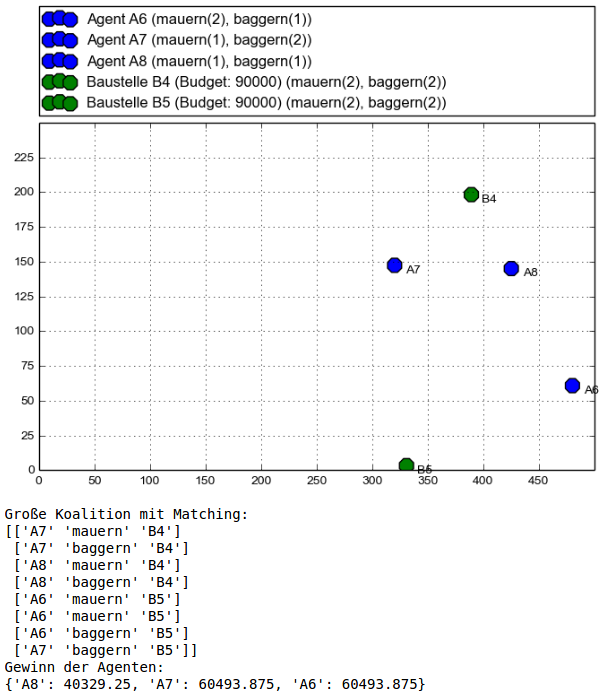
\includegraphics[width=0.5\textwidth]{example-shapley-value.png}
  \caption{Matching der großen Koalition und Gewinnverteilung.}
  \label{example-shapley-value}
\end{figure}

Für diese wird zunächst die Erlösverteilung nach dem Shapley Value und das dazugehörige Matching berechnet. In Abbildung \ref{example-shapley-value} ist dazu das Ergebnis zu einem Beispielszenario zu sehen. Im zweiten Schritt wird die Auktion für alle Szenarien durchgeführt.

\TODO{Grafik einbinden}

Die Ergebnisse sind in der Abbildung \ref{} zu sehen und entsprechen der Erwartung: ...

